\documentclass[11pt]{article}
\usepackage{graphicx}
\graphicspath{{images/}}
\usepackage{listings}
\usepackage{color}
\usepackage[utf8]{inputenc}
\usepackage{float}
\usepackage{siunitx}
\usepackage{tabto}
\usepackage{caption}
\usepackage{multirow}
\usepackage{pdfpages}
\usepackage[titletoc,toc]{appendix}
\usepackage[hidelinks]{hyperref}

\usepackage{fancyhdr}
\usepackage{amsmath}
\usepackage{subcaption}

\fancyhf{}
\setlength{\headheight}{0pt}
\renewcommand{\headrulewidth}{0pt}
\pagestyle{fancy}
\pagenumbering{gobble}

\definecolor{comment}{rgb}{0,0.6,0}
\definecolor{code}{rgb}{0.58,0,0.82}

\lstset{
	backgroundcolor=\color{white},
	commentstyle=\color{comment},
	frame=tb,
	keywordstyle=\color{blue},
	stringstyle=\color{code},
	language=C,
	basicstyle={\small\ttfamily}
}
\title{\textbf{ESP8266 WiFi extension Design}}
\author{Virgile Neu}
\date{\today \\ version 1.0}
\begin{document}
\maketitle
    \begin{figure}
        \center
        
\includegraphics[scale=0.9]{EPFL-Logo-CMJN.eps}
    \end{figure}
    \newpage
    
\tableofcontents

\newpage

\pagenumbering{arabic}
\setcounter{page}{1}
\lfoot{EPFL}
\cfoot{Virgile Neu}
\rfoot{\thepage}

\section{Introduction}

The ESP8266 chip is a WiFi module with a AT command mode. It can be used for 
single connection or multiple connections (server), either TCP or UDP.\\
It has 4 pins of interest plus \texttt{VCC} and \texttt{GND} : \texttt{Chip Enable}, \texttt{RESET}, \texttt{Rx} and \texttt{Tx}. The picture \ref{esp8266} below show the esp8266 board with it's connectivity.
\begin{figure}[H]
\centering
\begin{subfigure}{.7\textwidth}
  \centering
  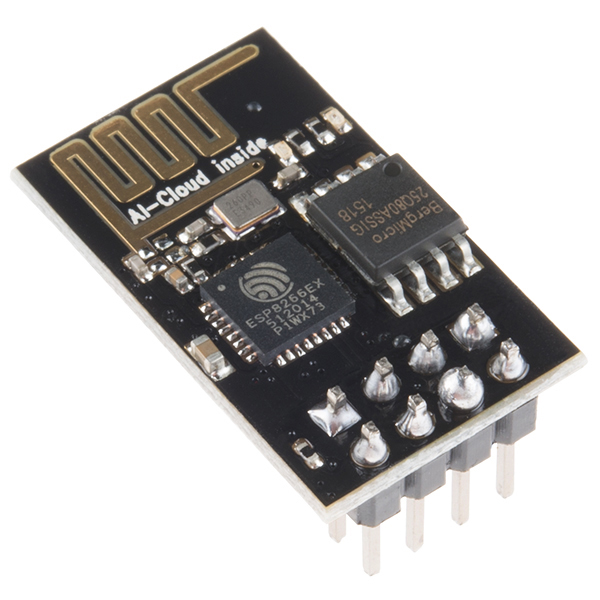
\includegraphics[width=.7\linewidth]{ESP8266.jpg}
\end{subfigure}%

\begin{subfigure}{.9\textwidth}
  \centering
  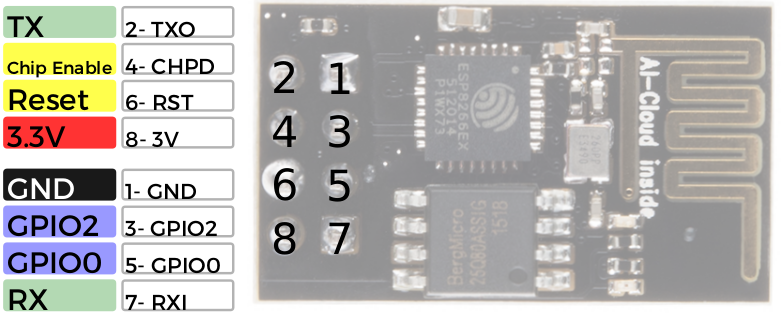
\includegraphics[width=.9\linewidth]{ESP8266_pinout.png}
\end{subfigure}
\caption{The ESP8266 module}
\label{esp8266}
\end{figure}

The goal is to make available this WiFi module to use on the FPGA and to make it easily usable.
\newpage
\section{Parameters}
\subsection{Default configuration}
The default configuration depends on the firmware version and can be changed at any time by AT commands with the \texttt{\_DEF} modifier (e.g. \texttt{AT+UART\_DEF}).\\
Most of the parameters can be set that way, or customise at run time without changing the stored settings with the \texttt{\_CUR} command modifier.
\subsection{Serial Parameters}
The ESP8266 WiFi module uses \texttt{UART} communication to transmit information with the FPGA.\\
The UART works as described on figure \ref{UART_data_transfert}. It starts with the start bit, always '0', then comes the data (here 8 bits), least significant bit first, then the parity bit (if set), and then 1 or 2 stop bit, always '1'.\\
The ESP8266 supports a lot of different settings :
\begin{figure}[H]
        \makebox[\textwidth][c]{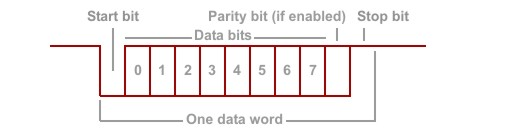
\includegraphics[width=\textwidth,height=\textheight,keepaspectratio]{uart_data.jpg}}
        \caption{UART data transfert.}
        \label{UART_data_transfert}
\end{figure}

\subsubsection{Data bits}
\begin{itemize}
    \item 5 bits
    \item 6 bits
    \item 7 bits
    \item 8 bits
\end{itemize}
\subsubsection{Baud rates}
Unlike the HC05, it supports a continuous range of baud rates, between 300 to 115200*40 bits/s.

\subsubsection{Stop bit}
\begin{itemize}
    \item 1 bit
    \item 1.5 bit
    \item 2 bit
\end{itemize}

\subsubsection{Parity bit}
\begin{itemize}
    \item None
    \item \texttt{Odd} parity
    \item \texttt{Event} parity
\end{itemize}

\subsubsection{Flow control}
\begin{itemize}
    \item No flow control
    \item enable \texttt{Request To Send}
    \item enable \texttt{Clear To Send}
    \item enable both \texttt{RTS} and \texttt{CTS}
\end{itemize}

The ESP8266 has on chip \texttt{Tx/Rx} FIFO of 128 Bytes.

\subsection{WiFi Parameters}
\subsubsection{Router connection}
It can connect to routers with several security : 
\begin{itemize}
\item \texttt{OPEN},
\item \texttt{WEP},
\item \texttt{WPA\_PSK},
\item \texttt{WPA2\_PSK},
\item \texttt{WPA\_WPA2\_PSK}.
\end{itemize}
The connection to routers with the \texttt{WPA2\_Entreprise} security is not available 
with the current version of the AT command set.\\
\subsubsection{Connection mode}
The ESP8266 has three WiFi connection modes :
\begin{itemize}
    \item \texttt{Station} mode : Client only
    \item \texttt{SoftAP} mode : Server only
    \item \texttt{SoftAP} + \texttt{Station} mode
\end{itemize}

\section{Design Choices}
Here I will show how the extension will look like, see figure \ref{high_level}. It will consist of Four parts:
\begin{itemize}
    \item \texttt{Registers}, to store configuration, status and other things,
    \item A \texttt{FIFO\_OUT} to send data from the CPU to the \texttt{UART} custom interface,
    \item A \texttt{FIFO\_IN} to receive data from the \texttt{ESP8266},
    \item A custom \texttt{UART} interface to communicate to the \texttt{ESP8266}.
\end{itemize}
\begin{figure}[H]
    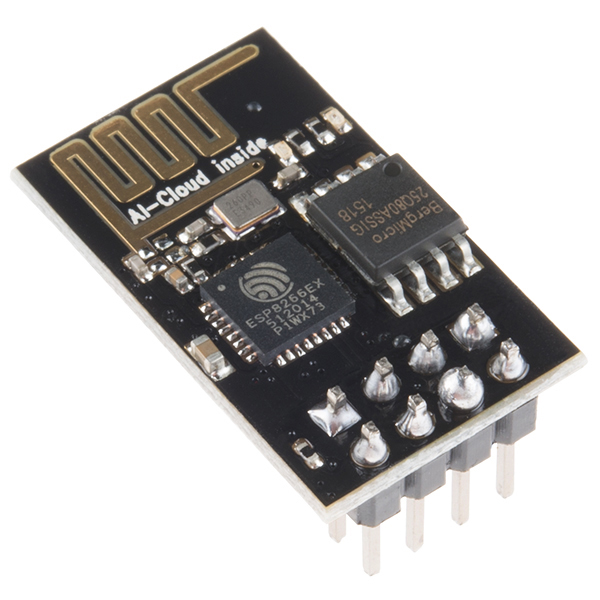
\includegraphics[width=.7\linewidth]{ESP8266.jpg}
    \caption{High level block diagram of the ESP8266 extension.}
    \label{high_level}
\end{figure}

\subsection{Registers}
The registers will have height registers :
\begin{itemize}
    \item A control register \texttt{CTRL},
    \item A status register \texttt{STATUS},
    \item A register for the \texttt{UART} waiting cycles (depends on the \texttt{UART rate}),
    \item The \texttt{FIFO\_out\_data} register,
    \item The \texttt{FIFO\_out\_free\_space} register,
    \item The \texttt{FIFO\_in\_data} register,
    \item The \texttt{FIFO\_in\_pending\_data} register.
    \item The \texttt{reset\_FIFO\_in} register.
\end{itemize}
Here is the register map in table \ref{reg_map} below.
\texttt{
\captionof{table}{Register map of the Registers component.}
\label{reg_map}
\centerline{
\begin{tabular}{|l|l|c|c|c|c|c|c|c|c|c|c|c|}
\hline
\# & addr & 31..8 & 7 & 6 & 5 & 4 & 3 & 2 & 1 & 0 & R/W\\
\hline
0 & 0x00 & \multicolumn{3}{c|}{Unused} & \multicolumn{3}{c|}{UART\_CTRL} & \multicolumn{2}{c|}{I\_ENABLE} & UART\_ON & R/W\\
\hline
1 & 0x04 & \multicolumn{7}{c|}{Unused} & \multicolumn{2}{c|}{i\_pending} & R/W\\
\hline
2 & 0x08 & \multicolumn{9}{c|}{UART\_wait\_cycles} & R/W\\
\hline
3 & 0x0C & ignored & \multicolumn{8}{c|}{FIFO\_out\_data} & W\\
\hline
4 & 0x10 & \multicolumn{9}{c|}{FIFO\_out\_free\_space} & R\\
\hline
5 & 0x14 & zeros & \multicolumn{8}{c|}{FIFO\_in\_data} & R\\
\hline
6 & 0x18 & \multicolumn{9}{c|}{FIFO\_in\_pending\_data} & R\\
\hline
7 & 0x1C & \multicolumn{7}{c|}{Unused} & Reset\_FIFO\_out & Reset\_FIFO\_in & W\\
\hline
\end{tabular}}
\begin{center}
\begin{tabular}{|c|c|c|}
\hline
\multicolumn{3}{|c|}{UART\_CTRL}\\
\hline
5 & 4 & 3\\
\hline
\multicolumn{2}{|c|}{Parity\_bit} & Stop\_bit\\
\hline
\end{tabular}
\begin{tabular}{|c|c|}
\hline
\multicolumn{2}{|c|}{I\_ENABLE}\\
\hline
2 & 1\\
\hline
i\_dropped & i\_received\\
\hline
\end{tabular}
\end{center}
}
The role of each bit is described below :
\begin{itemize}
    \item 0x00 :
    \begin{itemize}
        \item \texttt{UART\_ON} : Specifies if the \texttt{UART} will capture or send data or if it will stay off.
        \item \texttt{i\_reveived} : Specifies if the device can send interrupts request when receiving data from the \texttt{ESP8266}.
        \item \texttt{i\_dropped} : Specifies if the device can send interrupts request when some data is dropped.
        \item \texttt{stop\_bit} : Specifies the number of stop bit, '0' for 1, '1' for 2.
        \item \texttt{parity\_bit} : Specifies the parity bit, "00" for \texttt{None}, "10" for \texttt{Even} and "11" for \texttt{Odd}.
    \end{itemize}
    \item 0x04 : 
    \begin{itemize}
        \item \texttt{i\_pending} : Tells if there is an interrupt waiting to be served by the CPU. The CPU must clear it by software when serving the interrupt. Bit 0 is for i\_received, bit 1 is for i\_dropped. Writing '1' to any of the two bits has no effect.
    \end{itemize}
    \item 0x08 : \texttt{UART\_wait\_cycles} : Specifies to the \texttt{UART} how many cycles it should wait before capturing the values during the transfer. The values to put are described in the table \ref{UART_wait_cycles} below for a 50MHz clock. 
    \item 0x0C : \texttt{FIFO\_out\_data} : Address to write to send data to the \texttt{ESP8266} through the \texttt{FIFO\_out}. The write must has the \texttt{byte\_enable} signal equal to "0001".
    \item 0x10 : \texttt{FIFO\_out\_free\_space} : Number of free words (8 bits) in the \texttt{FIFO\_out}. 
    \item 0x14 : \texttt{FIFO\_in\_data} : Address to read to receive data from the \texttt{ESP8266} through the \texttt{FIFO\_in}. 
    \item 0x18 : \texttt{FIFO\_out\_free\_space} : Number of waiting words (8 bits) in the \texttt{FIFO\_in}. 
    \item 0x1C :
    \begin{itemize}
        \item \texttt{Reset\_FIFO\_in} : Write only bit to clear the \texttt{FIFO\_in}.
        \item \texttt{Reset\_FIFO\_out} : Write only bit to clear the \texttt{FIFO\_out}.
    \end{itemize}
\end{itemize}
\newpage
The value to put in the \texttt{UART\_wait\_cycles} registers depend on the desired \texttt{UART baud rate}, and is computed with the following formula.
\begin{align*}
wait\_cycles &= \frac{time\_per\_bit}{time\_per\_cycles}\\
&= \frac{\frac{1}{baud\_rate}}{clk\_period} \\
&= \frac{clk\_freq}{baud\_rate}
\intertext{For 4800 bits/s of baud rate we have.}
wait\_cycles &= \frac{clk\_freq}{baud\_rate}\\
&= \frac{50\cdot 10^{6}}{4800} = 10416.667 \quad clk\_cycles
\end{align*}
The rounding doesn't matter.
\captionof{table}{UART\_wait\_cycles values for a given UART.}
\label{UART_wait_cycles}
\begin{center}
\begin{tabular}{|l|r|}
\hline
UART\_Rate & wait\_cycles value (decimal)\\
\hline
4800 bits/s & 10416 clk\_cycles\\
\hline
9600 bits/s & 5207 clk\_cycles\\
\hline
19200 bits/s & 2604 clk\_cycles\\
\hline
38400 bits/s & 1302 clk\_cycles\\
\hline
57600 bits/s & 868 clk\_cycles\\
\hline
115200 bits/s & 434 clk\_cycles\\
\hline
230400 bits/s & 217 clk\_cycles\\
\hline
460800 bits/s & 109 clk\_cycles\\
\hline
921600 bits/s & 54 clk\_cycles\\
\hline
1382400 bits/s & 36 clk\_cycles\\
\hline
\end{tabular}
\end{center}

The ports of the Registers component are described on figure \ref{reg_ports} below.
\begin{figure}[H]
        \makebox[\textwidth][c]{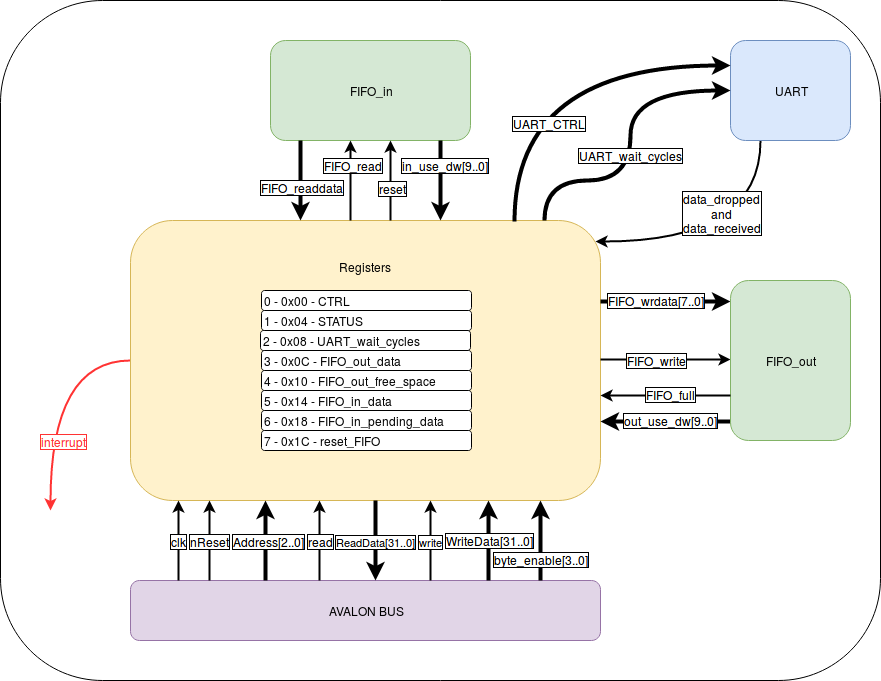
\includegraphics[width=\textwidth, height=\textheight,keepaspectratio]{registers_ports.png}}
        \caption{Ports description of the Registers component.}
        \label{reg_ports}
\end{figure}

\subsection{FIFO\_out}
For the FIFO\_out we will use the FIFO available in the IP catalogue of Quartus with the following configurations :
\begin{itemize}
    \item Width = 8 bits,
    \item Depth = 1024 (biggest size with only one M10k element),
    \item control signals : \begin{itemize}
        \item use\_dw[] (10 bits),
        \item empty,
        \item asynchronous clear; \end{itemize}
    \item Show ahead FIFO mode,
    \item Auto memory block type,
    \item No optimisation or circuitry protection.
\end{itemize}

The ports of the FIFO\_out component are described on figure \ref{fifo_out_ports}.
\begin{figure}[H]
        \makebox[\textwidth][c]{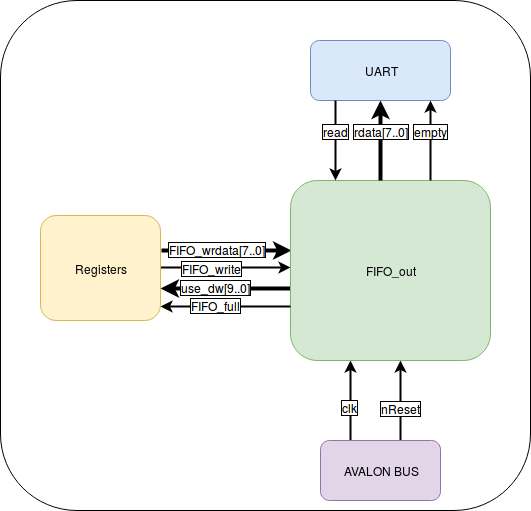
\includegraphics[width=\textwidth, height=\textheight,keepaspectratio]{FIFO_out_ports.png}}
        \caption{Ports description of the FIFO\_out component.}
        \label{fifo_out_ports}
\end{figure}

\subsection{FIFO\_in}
For the FIFO\_in we will also use the FIFO available in the IP catalogue of Quartus with almost the same configurations :
\begin{itemize}
    \item Width = 8 bits,
    \item Depth = 1024 (biggest size with only one M10k element),
    \item control signals : \begin{itemize}
        \item use\_dw[] (10 bits),
        \item full,
        \item asynchronous clear; \end{itemize}
    \item Normal synchronous FIFO mode,
    \item Auto memory block type,
    \item No optimisation or circuitry protection.
\end{itemize}

The ports of the FIFO\_in component are described on figure \ref{fifo_in_ports}.
\begin{figure}[H]
        \makebox[\textwidth][c]{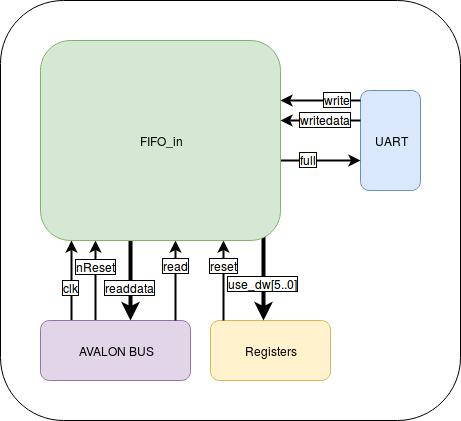
\includegraphics[width=\textwidth, height=\textheight,keepaspectratio]{FIFO_in_ports.png}}
        \caption{Ports description of the FIFO\_in component.}
        \label{fifo_in_ports}
\end{figure}

\subsection{UART}
The UART will be the part communicating with the ESP8266 module. It will send whenever it can while the FIFO\_out isn't empty, and whenever it receives information, it will recompose the words, perform the parity check (if set) and send the correct words to the FIFO\_in.
\\
The ports of the UART component are described on figure \ref{uart_ports}.
\begin{figure}[H]
        \makebox[\textwidth][c]{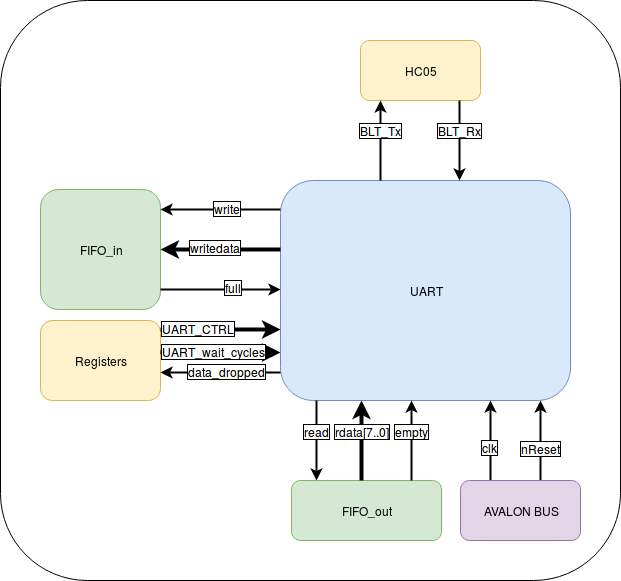
\includegraphics[width=\textwidth, height=\textheight,keepaspectratio]{UART_ports.png}}
        \caption{Ports description of the UART component.}
        \label{uart_ports}
\end{figure}

\section{Pinout}
The external connectivity of the device is described on table \ref{pinout}.
\begin{center}
\captionof{table}{Pinout table of the device.}
\label{pinout}
\begin{tabular}{|c|c|}
\hline
signal name & connectivity\\
\hline
\texttt{BLT\_RxD} & \texttt{GPIO\_0 23 -- FPGA PIN\_T11}\\
\hline
\texttt{BLT\_TxD} & \texttt{GPIO\_0 25 -- FPGA PIN\_AF6}\\
\hline
\texttt{BLT\_State} & \multirow{3}{*}{\texttt{PCA9673} via Avalon Bus}\\
\cline{1-1}
\texttt{BLT\_EN} &\\
\cline{1-1}
\texttt{BLT\_ATSel} &\\
\hline
\end{tabular}
\end{center}

\section{States Machines}
This section describes the several states machines used in the extension.
\subsection{UART}
\subsubsection{Transmitting State Machine}
The figure \ref{UART_transmit_SM} below describe the state machine used for transmitting data. It consists of 5 states : WAITING, START, SENDING, PARITY and STOP states. It starts at the WAITING states, and wait for data to be available in the FIFO\_out. Once data is available, it issue a read to the FIFO\_out and go to the start states. During the start state, it outputs the '0' value, as specified in the UART protocol, and store the data from the FIFO\_out\_readdata during the first cycle in this state. Once it has waited enough, it goes to sending. During sending state, it will send bit after bit, every time waiting the good amount of time. Oncei all the 8 bit of data are sent, it will either go to STOP if the parity is disabled (Parity\_bit = "00") or to PARITY if it is enable. In the PARITY state, it will output the parity value (odd or even) for the right amount of time, and then go to the STOP state. In the STOP state, it will output 1 or 2 bit at '1', depending on the settings of the Stop\_bit, and then go to the WAITING state, ready to transfer again.
\begin{figure}[H]
    \center
    \makebox[\textwidth][c]{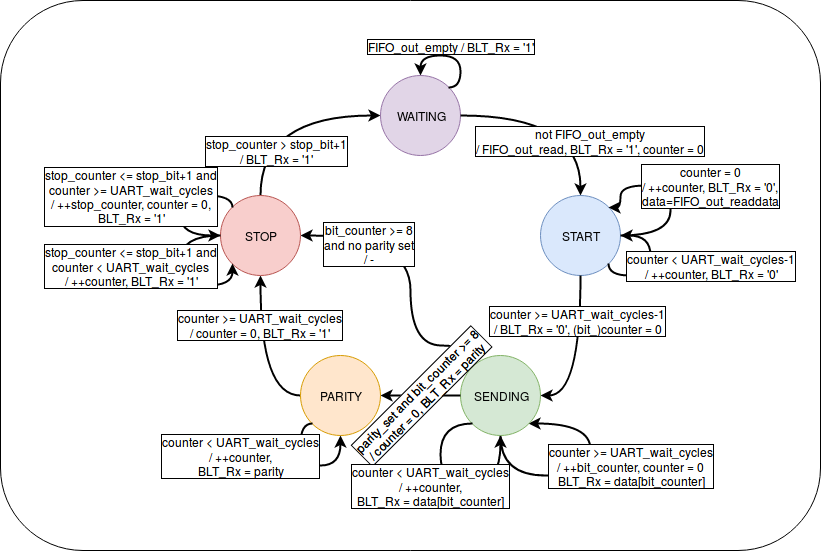
\includegraphics[width=\textwidth, height=\textheight,keepaspectratio]{UART_transmit_SM.png}}
    \caption{State machine used for sending one word (8 bits) to the ESP8266.}
    \label{UART_transmit_SM}
\end{figure}
\subsubsection{Receiving State Machine}
The figure \ref{UART_receive_SM} below describe the state machine used for receiving data. It has 4 states : WAITING, START, RECEIVING and PARITY. It starts at the WAITING states, and wait until the BLT\_Tx is '0' (start bit). Then we wait for half the cycles to wait in the START state in order to capture each bit in correctly and not just when they are supposed to go up (in order to avoid wrong bits), continuously checking that the start bit is still on (BLT\_Tx = '0'). Then we go to the RECEIVING state, where we wait for a full wait before capturing each bit. There is a transition back to the WAITING state with a big condition, it is to catch an error in the start bit during the first half of the first wait round. Once we received all the bits, we either go to the parity check in the PARITY state if enable or directly to the WAITING state and writing the data to the FIFO\_in if it is not full. If we go to the PARITY state, we check if the parity of the data we received is correct, and if it is we write it to the FIFO\_in if it is not full, and else we discard it. Then we go back to WAITING.
\begin{figure}[H]
    \makebox[\textwidth][c]{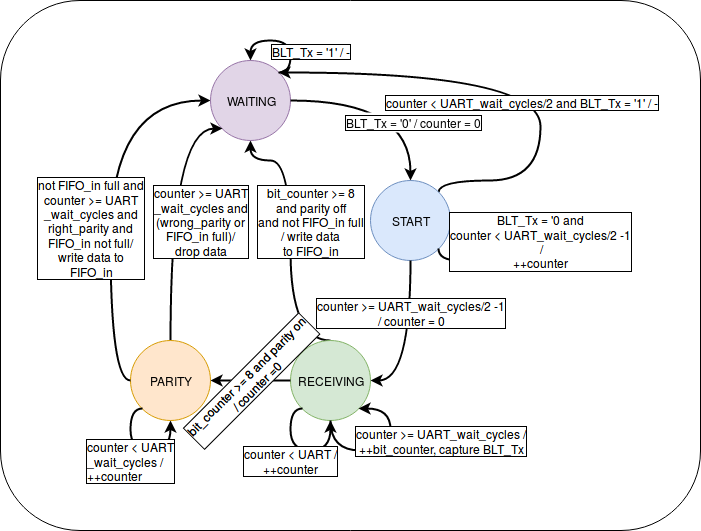
\includegraphics[width=\textwidth, height=\textheight,keepaspectratio]{UART_receive_SM.png}}
    \caption{State machine used for receiving one word (8 bits) from the ESP8266.}
    \label{UART_receive_SM}
\end{figure}

\section{Power consumption}
The \texttt{ESP8266} module specification document has the following table regarding power consumption:
\begin{figure}[H]
    \makebox[\textwidth][c]{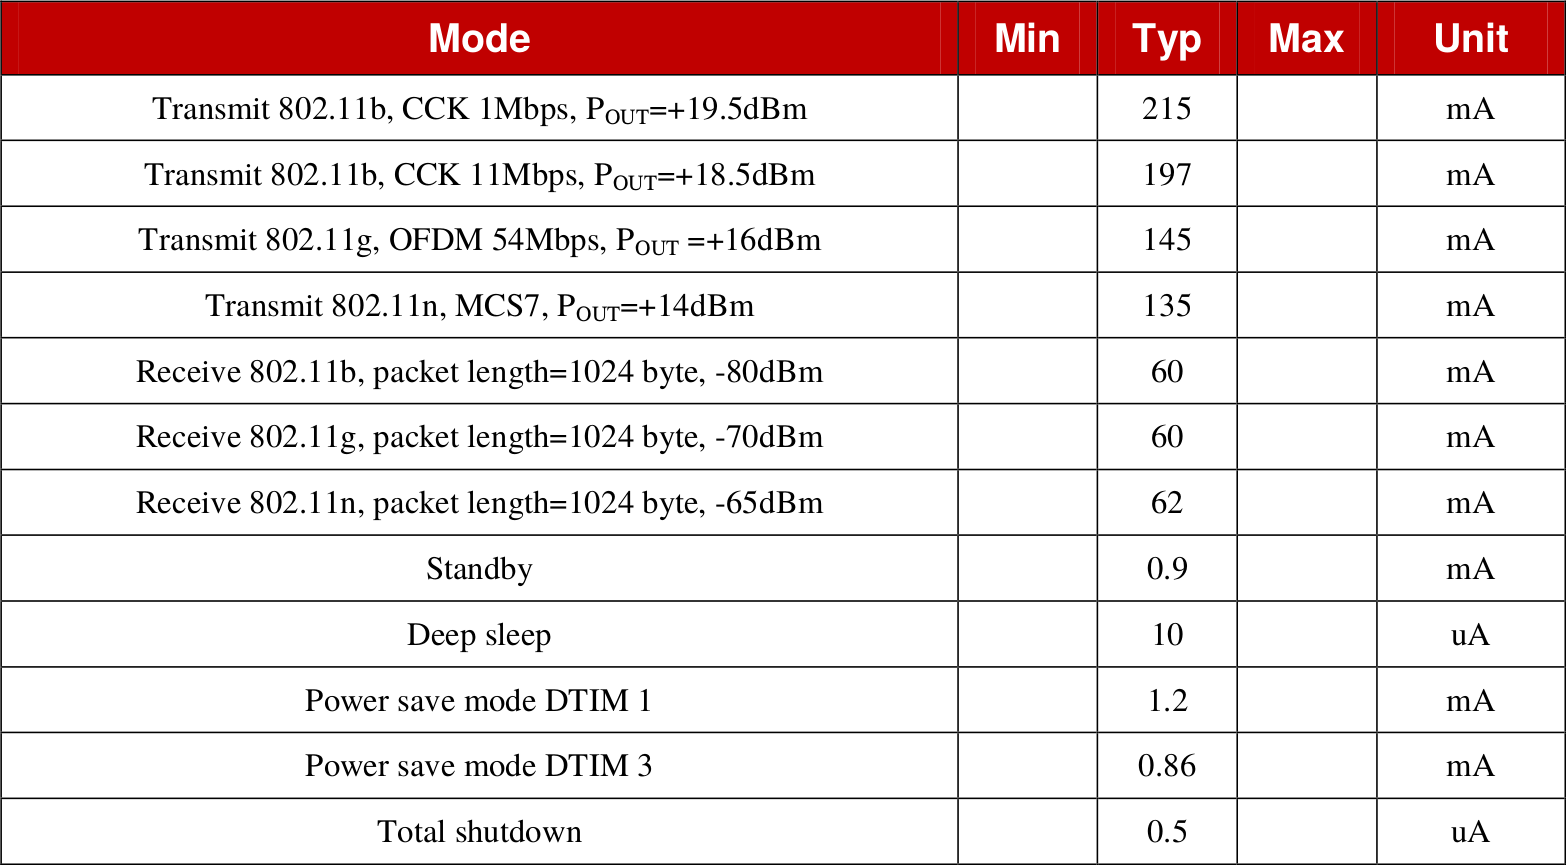
\includegraphics[width=\textwidth, height=\textheight,keepaspectratio]{powerConsumption.png}}
    \caption{Table with the power consumption of the module.}
\end{figure}

\section{Other}
The \texttt{ESP8266} module has a lot more to offer, since there is a real ARM 32 bit CPU inside with some GPIOs and ADCs for instance. All of that is not accessible as be only use it by UART without any SDKs, only with the AT commands. That way to use the module is sufficient to do some inter FPGA communication, or to access a remote server, but if one wants to use the SPI, ADC or many other things, he will have to flash another firmware with an SDK.
\newpage
\begin{appendices}
\section{Flashing the ROM}
In order to use the AT commands, you need to flash the ROM to update the software. This document was written for the version of the software given in archive with this file.\\
In order to correctly flash your module, please refer to the other pdf "\texttt{Flash\_ESP8266\_WiFi\_module.pdf}".
\section{AT Commands}
Below you can find the section from the \texttt{ESP8266} instruction manual regarding the AT commands.
\includepdf[pages={7-18}, scale=.82, pagecommand={}]{4a-esp8266_at_instruction_set_en.pdf}
\includepdf[pages={19-40}, scale=.82, pagecommand={}]{4a-esp8266_at_instruction_set_en.pdf}
\includepdf[pages={41-56}, scale=.82, pagecommand={}]{4a-esp8266_at_instruction_set_en.pdf}

\end{appendices}

\end{document}
